\documentclass[10pt]{article}
\usepackage[polish]{babel}
\usepackage[utf8]{inputenc}
\usepackage[T1]{fontenc}
\usepackage{amsmath}
\usepackage{amsfonts}
\usepackage{amssymb}
\usepackage[version=4]{mhchem}
\usepackage{stmaryrd}
\usepackage{graphicx}
\usepackage[export]{adjustbox}
\graphicspath{ {./images/} }

\title{KLASY PIERWSZE I DRUGIE }

\author{}
\date{}


\begin{document}
\maketitle
\begin{enumerate}
  \item Pewien hinduski maharadża pozostawił swoim sześciu synom w spadku sporą ilość wielkich diamentów jednakowej wartości, przy czym rozporządził, że pierwszy z synów weźmie jeden diament i \(\frac{1}{7}\) pozostałych, drugi - dwa diamenty i \(\frac{1}{7}\) pozostałych i tak dalej. Po dokonanym podziale okazało się, że każdy z synów otrzymał tę samą ilość diamentów. Ile było wszystkich diamentów?
  \item W zapisie
\end{enumerate}

\section*{1111111111}
wstaw między każde dwie jedynki znak działania (+,-, •, lub :) tak, aby uzyskać w wyniku kolejne liczby naturalne od 11 do 25. Można także używać nawiasów.\\
3. Dany jest pięciokąt foremny \(A B C D E\) i taki punkt \(P\) wewnątrz niego, że trójkąt \(A B P\) jest równoboczny. Jaka jest miara kąta \(B C P\) ?\\
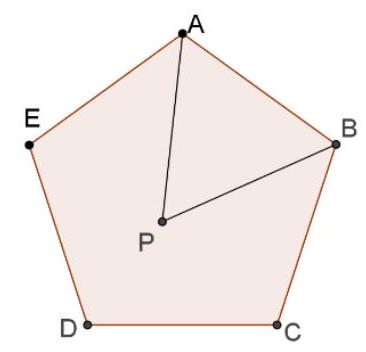
\includegraphics[max width=\textwidth, center]{2024_11_21_b77241a6b92a9bb65e10g-1}

\section*{KLASY TRZECIE I CZWARTE}
\begin{enumerate}
  \item Na półsferze o promieniu \(R\) leżą dwa styczne do siebie okręgi o promieniu \(r\). Wyznacz największą odległość między dwoma punktami należącymi do tych okręgów.
  \item Oblicz pole trójkąta, mając dane dwie proste \(4 x+5 y+17=0\) i \(x-3 y=0\), zawierające środkowe trójkąta, oraz jeden jego wierzchołek \(A=(-1,-6)\).
  \item Rozwiąż równanie:
\end{enumerate}

\[
\binom{n+1}{m+1}:\binom{n+1}{m} \frac{1}{n-m+1}=\frac{1}{3!}
\]

\(\operatorname{gdzie}\binom{n}{k}=\frac{n!}{k!(n-k)!}\)


\end{document}